\documentclass[conference]{IEEEtran}
\usepackage[T1]{fontenc}
\renewcommand{\ttdefault}{lmtt}
\usepackage{graphicx}
\usepackage{booktabs,tabularx,array}
\usepackage{amsmath}
\usepackage{csquotes}
\usepackage[numbers,sort&compress]{natbib}
\let\parencite\citep
\let\textcite\citet
\usepackage{xurl}
\usepackage[hidelinks]{hyperref}
\setlength{\emergencystretch}{2em}
\title{Interpretable Classification of Gallstone Status from Clinical and Bioimpedance Data: An Internal Validation Study}
\author{\IEEEauthorblockN{Duong Nguyen}\IEEEauthorblockA{University of Auckland}}
\date{}
\begin{document}
\maketitle
\begin{abstract}
This study compares interpretable and nonlinear classifiers for identifying existing gallstone status from demographic, laboratory, and bioimpedance measurements. A secondary analysis of 319 records with 38 candidate predictors evaluated logistic regression, random forest, XGBoost, LightGBM, and stacking using leave-one-patient-out (LOPO) internal validation, implemented as record-level leave-one-out under a one-record-per-person assumption. Imputation, recursive CART-based selection of 20 predictors, and transformation were fitted within training folds. Each model produced one held-out prediction per record. Logistic regression achieved the highest pooled ROC--AUC (0.874), whereas random forest achieved the highest accuracy (0.799), sensitivity (0.839), and F1 (0.808) among predictive models. Stacking achieved the highest specificity (0.772). These results distinguish discrimination from classification at the fixed threshold of 0.5 and support logistic regression as an interpretable research baseline. Recurrent errors across model families indicate limitations beyond aggregate scores. A small single-source cohort, overlapping training folds, retrospective model comparison, and absent calibration and external validation restrict inference. The findings concern existing disease status and do not establish prospective prediction or clinical utility.

\end{abstract}
\begin{IEEEkeywords}
Gallstone classification, clinical tabular data, logistic regression, feature selection, internal validation.
\end{IEEEkeywords}

\section{Introduction}\label{sec:introduction}
Gallstone status has been studied in relation to demographic, metabolic, laboratory, and body-composition characteristics \parencite{lammert2016gallstones,esen2024early}. Combining these measurements presents a supervised classification problem in which predictive discrimination must be considered alongside missed cases, false positives, and model interpretability. A small clinical dataset also raises a methodological question: does additional model complexity provide a consistent advantage over a regularised linear baseline?

This study evaluates that question using the published UCI Gallstone dataset. The outcome is gallstones present at assessment; the analysis does not model time to disease onset. Its purpose is to compare candidate classifiers and investigate the robustness of their internal performance, rather than establish a deployable diagnostic system.

The study makes three contributions within this dataset: a comparison of five predictive model families under shared, training-specific preprocessing and RFE--CART feature selection; LOPO internal validation yielding one held-out prediction per record; and retrospective analysis of errors recurring across model families. The comparison distinguishes probability discrimination from sensitivity and specificity at a common decision threshold.


\section{Related Work}\label{sec:related-work}
\label{sec:literature_review}
\subsection{Non-imaging classification and feature reduction}
Clinical, biochemical, and bioimpedance measurements have been investigated as non-imaging predictors of existing gallstone status. \textcite{esen2024early} introduced Gallstone-1, comprising 319 participants (161 cases and 158 controls) and 38 predictors, now available through UCI \parencite{uci2025gallstone}. Among nine conventional classifiers, gradient boosting achieved the highest reported accuracy (85.42\%). Vitamin D, C-reactive protein (CRP), total body water, and lean mass emerged as important predictors. These findings support the predictive relevance of heterogeneous measurements and motivate nonlinear modelling and feature reduction; they do not establish prospective disease prediction.

Subsequent optimisation studies show that dimensionality reduction offers a more consistent benefit than increased accuracy. \textcite{sarker2025gallstone} compared random forest with and without Sand Cat Swarm Optimization, under holdout and ten-fold cross-validation. Using 38 features, holdout accuracy, F1, precision, and recall were 81.25\%, 79.07\%, 85.00\%, and 73.91\%, respectively; mean cross-validation accuracy was 78.42\%. Optimisation retained 13 predictors, with 79.17\% holdout accuracy and 78.32\% cross-validation accuracy. Thus, approximately two thirds of the measurements were removed while maintaining similar performance. SHAP identified CRP, vitamin D, and aspartate aminotransferase as influential, while DiCE supplied individual counterfactual explanations.

\textcite{shrestha2026metaheuristic} combined Rotation Forest with Bald Eagle Search. The full-feature baseline achieved 78.00\% accuracy, 77.35\% F1, 79.33\% precision, 75.79\% recall, and approximately 0.867 AUC. Retaining 17 predictors reduced accuracy to 75.79\% and AUC to approximately 0.860. Near-perfect training performance contrasted with substantially lower test scores, indicating limited generalisation despite model complexity. SHAP and LIME highlighted CRP, vitamin D, obesity-related measurements, haemoglobin, and body mass. Feature reduction therefore simplified measurement requirements without improving discrimination.

\textcite{das2026sloa} reported a modest benefit from Sea Lion Optimization with CatBoost. Five-fold mean accuracy increased from 79.58\% to 80.42\% while the feature count fell from 38 to 19; F1 increased from 79.01\% to approximately 79.94\%, precision from 80.91\% to 81.97\%, and recall from 77.36\% to 77.76\%. Optimised fold accuracy ranged from approximately 71.88\% to 87.50\%, demonstrating sensitivity to partitioning. SHAP, LIME, and DiCE again emphasised CRP and vitamin D. Collectively, these studies favour assessing measurement burden, stability, and generalisation alongside headline accuracy.

\subsection{Consensus selection, ensembles, and probability assessment}
\textcite{tamer2026novel} combined four statistical selectors (minimum redundancy maximum relevance, chi-square, ANOVA, and Kruskal--Wallis) with four metaheuristics (Grey Wolf, Whale, Harris Hawks, and Particle Swarm optimisation). Agreement among at least seven selectors retained 11 predictors. Across nine classifiers, random forest achieved the highest reported accuracy (90.62\%); CRP, haemoglobin, vitamin D, and hyperlipidaemia remained in the subset. Consensus selection may identify complementary information and reduce redundancy, but its stability requires direct assessment. Selection informed by observations outside the training partition would yield optimistic estimates; repeated or nested validation is therefore necessary to evaluate the procedure reliably.

Hyperparameter optimisation provides a distinct route to improving performance. \textcite{rahman2026hbb} combined Bees Algorithm global search with Bayesian optimisation for XGBoost. HBB-Opt achieved 87.50\% accuracy, 87.49\% F1, 0.9258 ROC--AUC, 90.62\% sensitivity, and 90.00\% negative predictive value. A Brier score of 0.098 additionally assessed probabilistic accuracy, although this score alone does not establish calibration. SHAP highlighted CRP, vitamin D, obesity percentage, visceral fat area, and extracellular-fluid/total-body-water ratio. This work broadens evaluation beyond class labels to the quality of predicted probabilities.

\textcite{indirani2026ensemble} investigated stacking and soft voting across random forest, XGBoost, logistic regression, gradient boosting, Extra Trees, LightGBM, and support vector machines, incorporating SHAP selection, calibration, and threshold adjustment. Random-forest/XGBoost stacking with a logistic meta-learner achieved 85.94\% accuracy and 0.9307 AUC. Soft-voting accuracy increased from 79.69\% at the default threshold to 87.50\% after validation-based adjustment, with approximately 94\% positive-class recall. SHAP-based selection achieved approximately 0.9238 AUC and the same adjusted accuracy. These results distinguish probability ranking from operating-point decisions: strong AUC or accuracy does not necessarily imply adequate sensitivity. Threshold selection must remain within development data, and calibration requires separate evaluation.

\subsection{Synthesis and study positioning}
Across these studies, tree-based ensembles capture useful predictive patterns, but additional optimisation does not consistently improve generalisation. CRP, vitamin D, and body-composition measurements recur across attribution and selection analyses, supporting their predictive relevance within this cohort. Such recurrence is not independent biological validation: most studies reuse the same 319 observations, and neither attribution nor counterfactual explanation establishes causality. Near-perfect training results in random forest, Rotation Forest, and CatBoost further highlight overfitting risk when predictors are numerous relative to sample size.

Differences in partitions, selection procedures, search budgets, and thresholds preclude ranking methods directly from published scores. Larger independent cohorts remain necessary to establish transferability, calibration, and clinical utility. The present study consequently compares an interpretable logistic-regression baseline with nonlinear and stacked alternatives under a shared, training-fitted pipeline and leave-one-patient-out (LOPO) evaluation. Accuracy, AUC, sensitivity, specificity, F1, and false-negative behaviour characterise complementary aspects of performance. LOPO supplies one held-out prediction per record while retaining almost the entire small cohort for training; it provides internal validation rather than resolving external generalisation or model-selection bias.


\section{Materials and Methods}\label{sec:methods}
\subsection{Dataset and outcome}
The analysis used 319 records from the UCI Gallstone dataset, originating from a clinical study at Ankara VM Medical Park Hospital, Turkey, conducted between June 2022 and June 2023 \parencite{esen2024early,uci2025gallstone}. The cohort comprises 161 gallstone cases, 158 controls, and 38 demographic, comorbidity, anthropometric, bioimpedance, and laboratory predictors. No new primary data were collected. Source status 0 was recoded as class 1 (gallstones present), so sensitivity refers to detection of gallstones. Source-row identifiers trace predictions and are excluded from predictors; they are not verified patient identifiers.

\subsection{Fold-specific preprocessing and feature selection}
Within each outer training fold, continuous variables were median-imputed and categorical variables mode-imputed. Recursive feature elimination with a classification and regression tree (RFE--CART) retained 20 source predictors, removing one feature per step. The selection tree used maximum depth 5 and minimum leaf size 4. Selected continuous variables underwent Yeo--Johnson transformation \parencite{yeo2000new} and standardisation; categorical variables were one-hot encoded.

Every learned preparation stage was fitted using training records only and then applied to the excluded record. For stacking, preprocessing and supervised selection were additionally refitted within each inner training fold used to construct meta-model inputs. The globally transformed reference CSV was not an evaluation input. This design prevents the excluded record from informing imputation, selection, or transformation.

\subsection{Fixed model configurations}
Five predictive families were evaluated: logistic regression, random forest, XGBoost, LightGBM, and stacking. A training-prior dummy classifier provided a feature-free benchmark. Preprocessing and baseline estimation used scikit-learn \parencite{pedregosa2011scikit}. Table~\ref{tab:python-parameters} summarises the implemented fixed settings. The fixed benchmark used these settings without hyperparameter search; the additional nested tuning procedure is described below.

\begin{table}[tbp]
\centering
\small
\caption{Fixed configurations used in the Leave One Patient Out comparison. Random-state settings used seed 42.}
\label{tab:python-parameters}
\begin{tabularx}{\linewidth}{@{}p{2.7cm}X@{}}
\toprule
Model & Configuration \\
\midrule
Logistic regression & $C=1$; maximum 3,000 iterations. \\
Random forest & 60 trees; maximum depth 5; minimum leaf size 4. \\
XGBoost & 60 trees; learning rate 0.05; depth 2; $\lambda=1$; row and column sampling 0.8; histogram tree method. \\
LightGBM & 60 trees; learning rate 0.05; 7 leaves; minimum child samples 20; column sampling 0.8. \\
Stacking & Four individual classifiers as base learners; three stratified inner folds; probability inputs to a standardised logistic meta-model ($C=1$, maximum 3,000 iterations); no raw-feature passthrough. \\
Training-prior dummy & Class probabilities estimated from the outer training fold. \\
\bottomrule
\end{tabularx}
\end{table}

\subsection{Leave One Patient Out Evaluation Protocol}
LOPO was the sole evaluation strategy reported in this study. For each record $i$, the entire pipeline was fitted on the remaining 318 records and generated a probability $\hat{p}_i$ for the excluded record. Repeating this process across all 319 records produced exactly one out-of-fold prediction per record and per model. The implementation uses record-level leave-one-out cross-validation; it is equivalent to leave-one-patient-out only under the assumption that each record represents a distinct person. Repeated observations from the same person would instead require grouped exclusion.

Metrics were computed from the pooled out-of-fold predictions, rather than averaged over single-record folds. ROC--AUC measured discrimination, while accuracy, sensitivity, specificity, precision, F1, and false-negative rate characterised classification at the fixed threshold $\hat{p}_i\geq0.5$. False-negative rate was defined as $\mathrm{FN}/(\mathrm{TP}+\mathrm{FN})$. Pooling is necessary because a single excluded observation cannot support a fold-level AUC or a complete confusion matrix. Seed 42 controlled estimator randomness and stacking's stratified inner folds; the outer LOPO partitions themselves are deterministic.

Each fixed pipeline was assessed separately. Selecting the highest-scoring family retrospectively does not provide an unbiased estimate of a subsequent model-selection procedure: that would require nesting selection within each outer training fold. The 319 folds have heavily overlapping training sets and are not independent replications. A single LOPO run therefore supplies neither between-seed variance nor evidence of statistically significant model differences. No threshold optimisation, dedicated calibration assessment, or external validation was performed.

\subsection{Nested Optuna Hyperparameter Tuning}
For each excluded record and each predictive family, Optuna conducted 20 sequential trials on the remaining 318 records. A seeded tree-structured Parzen estimator maximised mean ROC--AUC across three stratified inner folds. Each trial refitted imputation, RFE--CART, transformation, and classification within the inner training folds. The best tested configuration was then refitted on all 318 outer training records to predict the excluded record. The feature count remained 20 and the classification threshold remained 0.5. Each family was tuned separately; model-family selection was not included within the outer evaluation.

Logistic regression searched $C\in[0.01,100]$ on a logarithmic scale. Random forest searched 40--160 trees (step 20), depth 2--8, minimum leaf size 2--10, and feature sampling from $\{\text{sqrt},0.5,1.0\}$. XGBoost and LightGBM searched 40--160 trees, learning rate 0.01--0.15, column sampling 0.6--1.0, and $\lambda$ 0.1--10; learning rate and regularisation used logarithmic sampling. XGBoost additionally searched depth 1--4 and row sampling 0.6--1.0. LightGBM searched 3--15 leaves and minimum child samples 10--40. Stacking searched only the logistic meta-learner's $C$ over 0.01--100, with the four base learners fixed. The prior dummy was not tuned.

Completed trial histories, best parameters, excluded-record predictions, configuration metadata, and fold checkpoints were saved separately from historical fixed results. Tuned runs used Optuna 5.0.0, scikit-learn 1.9.1, NumPy 2.5.3, pandas 3.0.6, XGBoost 3.4.1, and LightGBM 4.7.0. This nested design excludes the outer record from parameter selection, but does not eliminate optimism associated with prior dataset exploration or retrospective choice among model families.

\subsection{Error analysis and reproducibility}
Saved out-of-fold probabilities, labels, and source-row identifiers supported retrospective comparison of false negatives and false positives across model families. Records repeatedly misclassified by different families were treated as descriptive examples, not evidence of mislabelling, causal mechanisms, or future error prevalence. After evaluation, each pipeline was refitted on all 319 records for persistence. These full-data models were not used to calculate the reported LOPO metrics. The saved configuration records the seed, selector, feature count, and dataset signature to link results to the evaluated data.

\subsection{Explainable Artificial Intelligence (XAI) Analysis}
Explainable artificial intelligence (XAI) was used to examine feature contributions and classification errors. Both Kernel SHAP and LIME explained the Optuna-tuned logistic regression pipeline (fold-specific imputation, RFE--CART selection, transformation, encoding, and classification), which had the highest pooled AUC among the completed Optuna-tuned families (0.868). Explanations reconstructed the selected pipeline for each excluded record and verified its probability against the saved outer prediction. Thus, these figures concern the tuned model rather than the fixed configurations in Table~\ref{tab:building-lopo-results}. Selecting logistic regression for interpretation after inspecting outer scores is retrospective and does not evaluate a nested family-selection procedure.

Kernel SHAP \parencite{lundberg2017shap} explained the complete raw-feature pipeline in probability units using 25 background records drawn only from the relevant outer training fold and 256 perturbation samples. A fixed random sample of 20 excluded records supported the global summary; each record was explained with its own fold model and background. LIME \parencite{ribeiro2016lime} used 3,000 perturbations, training-only categorical frequencies and continuous discretisation, and eight displayed conditions. The most confident false negative and false positive were selected retrospectively for local illustration. Local surrogate $R^2$ was reported to assess fidelity. The explained output was the probability of gallstones present (class 1). Kernel SHAP and LIME are explanation methods applied to this predictive pipeline; the LIME surrogate is used only to approximate local behaviour. Attributions quantify fitted model behaviour rather than causal or clinically validated effects.


\section{Results}\label{sec:results}
\subsection{Fixed-Parameter Leave One Patient Out Benchmarks}
Logistic regression achieved the highest pooled AUC (0.874), while random forest achieved the highest accuracy (0.799), sensitivity (0.839), and F1 (0.808) among predictive models (Table~\ref{tab:building-lopo-results}). Logistic regression detected 132 of 161 positive records and correctly classified 118 of 158 controls; random forest detected 135 positive records and correctly classified 120 controls. Stacking had the highest specificity (0.772).

\begin{table*}[t]
\centering
\footnotesize
\caption{Fixed-parameter Leave One Patient Out evaluation on 319 held-out predictions per model at threshold 0.5.}
\label{tab:building-lopo-results}
\begin{tabular}{@{}lrrrrrr@{}}
\toprule
Model & Accuracy & ROC--AUC & Sensitivity & Specificity & F1 & FNR \\
\midrule
Logistic regression & 0.784 & \textbf{0.874} & 0.820 & 0.747 & 0.793 & 0.180 \\
Random forest & \textbf{0.799} & 0.857 & \textbf{0.839} & 0.759 & \textbf{0.808} & \textbf{0.161} \\
XGBoost & 0.762 & 0.835 & 0.807 & 0.715 & 0.774 & 0.193 \\
LightGBM & 0.787 & 0.851 & 0.832 & 0.741 & 0.798 & 0.168 \\
Stacking & 0.787 & 0.865 & 0.801 & \textbf{0.772} & 0.791 & 0.199 \\
\midrule
Training-prior dummy & 0.505 & 0.000 & 1.000 & 0.000 & 0.671 & 0.000 \\
\bottomrule
\end{tabular}
\end{table*}
The training-prior dummy's pooled AUC of 0.000 is a leave-one-out artefact: excluding a positive record lowers its training prevalence, while excluding a negative record raises it. Its pooled probabilities therefore rank the classes inversely, even though every thresholded prediction is positive. The value is not evidence of useful discrimination.

The single LOPO run compares fixed pipelines using the same excluded records; it does not estimate between-seed variability or the performance of a nested model-selection procedure.

\subsection{Optuna-Tuned Leave One Patient Out Benchmarks}
All five predictive families completed 319 outer folds with 20 Optuna trials and three stratified inner folds per outer training set. The source-data signature, feature count, seed, threshold, and dependency versions were identical across tuned runs. The first five rows of Table~\ref{tab:tuned-lopo-results} are these historical fixed-RFE20 runs; the final row is updated stacking with a searched feature count. All scores evaluate pooled held-out predictions, not inner validation scores.

\begin{table*}[t]
\centering\footnotesize
\setlength{\tabcolsep}{4pt}
\caption{Completed Optuna LOPO test results: 319 held-out predictions per configuration, seed 42, twenty trials, three inner folds and threshold 0.5. The first five rows use fixed RFE20; updated stacking searches k in 10/20/30/38 and tunes XGBoost/LightGBM/ridge bases with a fixed logistic meta learner. Bold marks the best observed value (lower for FNR/FN). Different search designs limit causal comparisons.}
\label{tab:tuned-lopo-results}
\begin{tabular}{@{}lrrrrrrrr@{}}
\toprule
Model/configuration & Accuracy & ROC--AUC & Precision & Sensitivity & Specificity & F1 & FNR & FN \\
\midrule
Logistic regression & 0.7868 & 0.8680 & 0.7688 & 0.8261 & 0.7468 & 0.7964 & 0.1739 & 28 \\
Random forest & 0.7743 & 0.8421 & 0.7602 & 0.8075 & 0.7405 & 0.7831 & 0.1925 & 31 \\
XGBoost & 0.7837 & 0.8509 & 0.7644 & 0.8261 & 0.7405 & 0.7940 & 0.1739 & 28 \\
LightGBM & 0.7868 & 0.8395 & 0.7751 & 0.8137 & 0.7595 & 0.7939 & 0.1863 & 30 \\
Stacking (historical, meta-tuned) & 0.7837 & 0.8617 & 0.7738 & 0.8075 & 0.7595 & 0.7903 & 0.1925 & 31 \\
\midrule
Stacking (updated, base-tuned) & \textbf{0.8056} & \textbf{0.8762} & \textbf{0.7895} & \textbf{0.8385} & \textbf{0.7722} & \textbf{0.8133} & \textbf{0.1615} & \textbf{26} \\
\bottomrule
\end{tabular}
\end{table*}

Within the historical fixed-RFE20 comparison, tuned logistic regression retained the highest AUC (0.868) and F1 (0.796), with accuracy 0.787 and sensitivity 0.826. It detected 133 of 161 cases and correctly classified 118 of 158 controls. XGBoost matched its sensitivity and false-negative count (28), but had lower AUC (0.851) and one additional false positive (41 versus 40). LightGBM matched the highest accuracy (0.787), while LightGBM and stacking shared the highest specificity (0.759). Random forest achieved AUC 0.842 and sensitivity 0.807. Stacking did not exceed logistic regression in discrimination or sensitivity; only its logistic meta-learner was tuned, with fixed base-model settings.

\subsection{Updated Base-Tuned Stacking with Joint Feature Selection}
The completed search-version-3 stacking run evaluated all 319 outer exclusions using seed 42, twenty Optuna trials per exclusion and three stratified inner validation folds. Unlike the historical meta-only search, this run jointly tuned XGBoost, LightGBM and ridge base learners and the RFE feature count; the standardised logistic meta-learner remained fixed at $C=1$. Table~\ref{tab:tuned-lopo-results} reports metrics recomputed from the saved outer predictions, not averages of inner validation scores.



The updated stack correctly classified 257 of 319 records: TN=122, FP=36, FN=26 and TP=135. Its AUC increased descriptively by 0.0145 and five fewer positive records were missed relative to the historical tuned stack. Across completed tuned experiments, this configuration has the highest observed AUC, accuracy, sensitivity, specificity and F1. These rankings are descriptive: the standalone candidates have not been rerun with the new feature-count search, and no significance or independent replication is established.

Optuna selected 10 features in one outer fold, 20 in 45 folds, 30 in 34 folds and all 38 in 239 folds. This favours the full input set in most exclusions and does not support a claim that a reduced twenty-field subset is optimal for the updated stack. The arithmetic mean selected-trial inner-validation AUC was 0.8747 across exclusions; it is a tuning diagnostic, not the outer test AUC, and its heavily overlapping validation sets are not independent replications.

The source evidence is \path{results/stacking_v3}: configuration, 319 prediction rows, 319 outer checkpoints, 6,380 completed Optuna trials and \path{CV_Metrics/stacking.csv}. The latter retains the selected trial's three-fold mean, sample standard deviation and individual-fold accuracy, AUC, precision, recall, specificity and sensitivity, plus selected feature count. Recall and sensitivity denote the same positive-class quantity. The new stack changes base composition, tuning scope, feature-count search and sampler-seed scheduling together; the observed improvement cannot be attributed to one change alone. SHAP/LIME figures below still explain the historical tuned logistic models and have not been regenerated for the new stack.

\subsection{Historical Changes Relative to Fixed Configurations}
XGBoost showed the largest positive change relative to its historical fixed benchmark: AUC increased from 0.835 to 0.851, accuracy from 0.762 to 0.784, and sensitivity from 0.807 to 0.826; false negatives decreased from 31 to 28. Logistic regression's AUC decreased from 0.874 to 0.868, although accuracy increased slightly and one fewer positive record was missed. Random forest's AUC decreased from 0.857 to 0.842, with five additional false negatives (26 to 31). LightGBM's accuracy was unchanged, but AUC decreased from 0.851 to 0.840 and false negatives increased from 27 to 30. Stacking's AUC decreased from 0.865 to 0.862; one fewer false negative was offset by two additional false positives.

These differences are descriptive rather than evidence that tuning alone caused the changes. The historical fixed run used scikit-learn 1.7.1, whereas the tuned runs used 1.9.1; NumPy and pandas versions also differed. Although the cohort and outer record exclusions were shared, a controlled estimate of tuning's effect requires refitting the fixed configurations in the tuned environment. No significance test or confidence interval was calculated. Optimising inner-fold AUC did not consistently improve outer discrimination or classification at threshold 0.5, and the search budget does not establish globally optimal parameters.


\subsection{Confusion Matrices and Average Classification Error}
Figure~\ref{fig:experimental-confusion} reproduces the saved fixed-parameter Experimental LOPO ROC/confusion-matrix figure and adds a descriptive mean confusion matrix across the five predictive families in Table~\ref{tab:building-lopo-results}, excluding the dummy. Mean counts were 118.0 true negatives, 40.0 false positives, 29.0 false negatives, and 132.0 true positives. The mean classification error was $(40+29)/319=21.6\%$, with mean false-negative rate $29/161=18.0\%$. This averages model-specific counts on the same 319 held-out records; it is not an ensemble confusion matrix, an average across seeds, or a set of independent replications. Tuned logistic regression, which is explained in the XAI results, instead had 118 true negatives, 40 false positives, 28 false negatives, and 133 true positives.

\begin{figure*}[t]
\centering
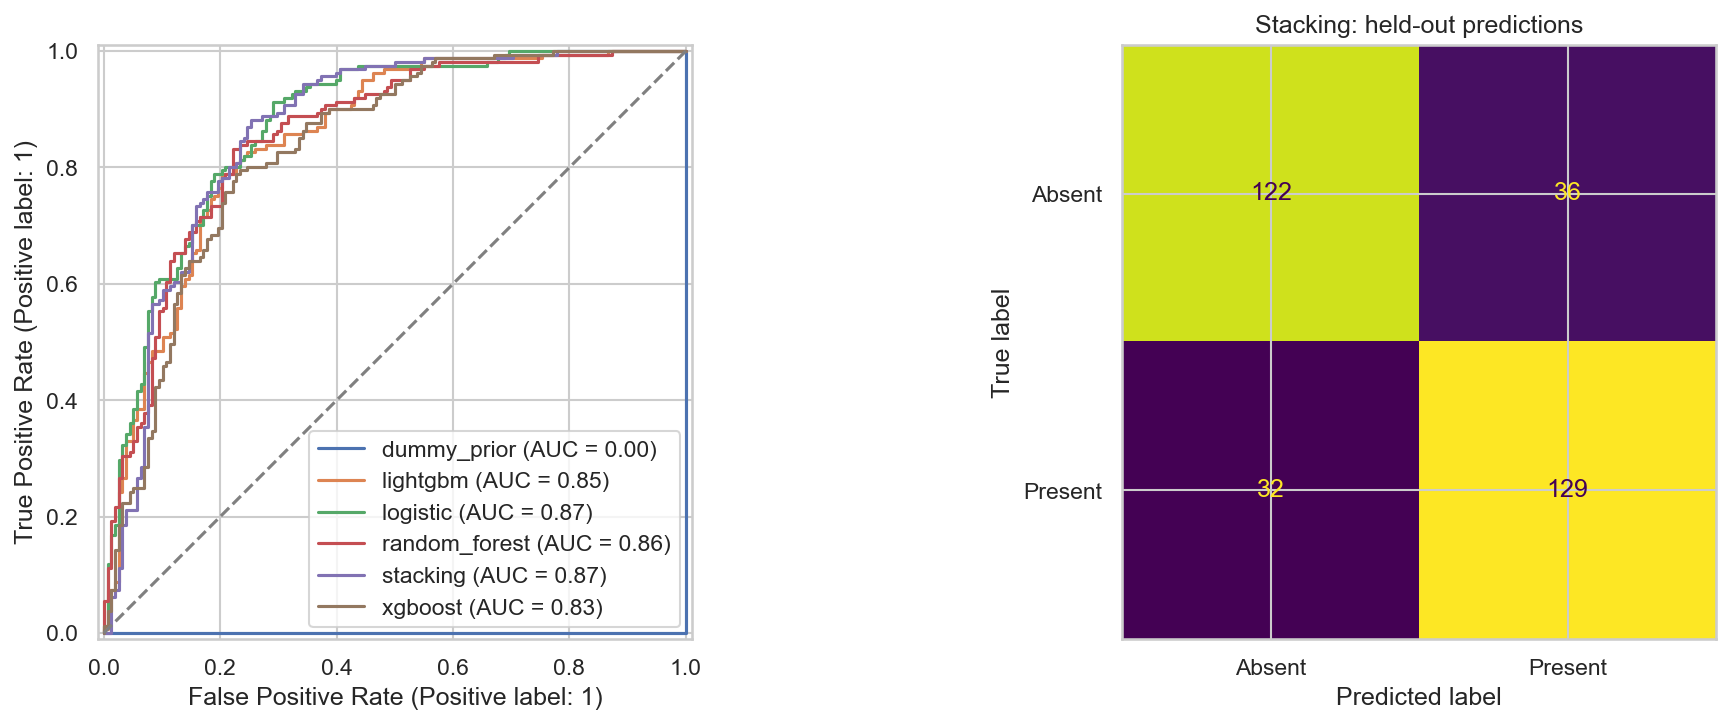
\includegraphics[width=0.97\linewidth]{figures/evaluation/experimental_lopo_roc_confusion.png}
\par\medskip
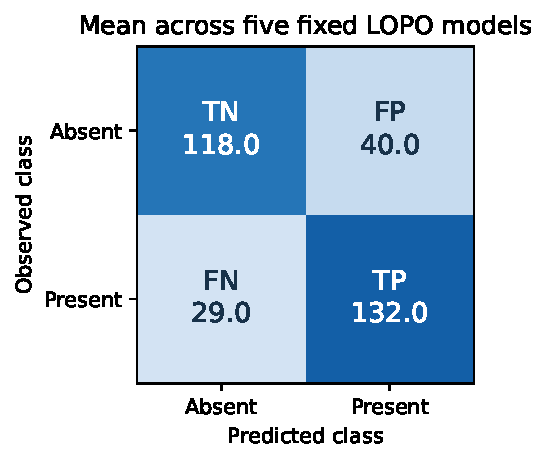
\includegraphics[width=0.43\linewidth]{figures/evaluation/average_fixed_lopo_confusion.pdf}
\caption{Fixed-parameter Experimental LOPO results at threshold 0.5. Top: existing ROC curves and the stacking confusion matrix (TN=122, FP=36, FN=32, TP=129). Bottom: arithmetic mean counts across logistic regression, random forest, XGBoost, LightGBM, and stacking, each evaluated on the same 319 records. The mean summarises model errors and does not represent predictions from a single classifier.}
\label{fig:experimental-confusion}
\end{figure*}

\subsection{Recurring Classification Errors in Fixed Models}
Source record 117 was a false negative in four of the five predictive LOPO models. Records 291 and 316 were false positives in all five. These retrospectively identified examples indicate disagreement between observed labels and predictions across model families, without establishing clinical causes or labelling errors. They support inspecting common failure cases in addition to aggregate discrimination and classification metrics.

\subsection{SHAP and LIME Explanations of Tuned Logistic Regression}
All XAI results in this subsection explain the Optuna-tuned logistic regression pipeline, using a separately fitted outer-fold model for each held-out record. The fixed logistic regression, random forest, XGBoost, LightGBM, and stacking benchmarks were not the models explained in these figures. Figure~\ref{fig:xai-global} summarises the 20 sampled held-out explanations from the tuned logistic models. The largest mean absolute SHAP contributions were associated with the source fields \texttt{bm} (0.208), CRP (0.173), extracellular-fluid/total-body-water ratio (0.071), vitamin D (0.068), weight (0.065), and extracellular water (0.056). The ordering describes this small sample and the fold-specific models, rather than a population-level ranking. Higher recorded CRP values generally contributed towards the absent class within these fitted models; this association does not imply a protective biological effect.

\begin{figure}[tbp]
\centering
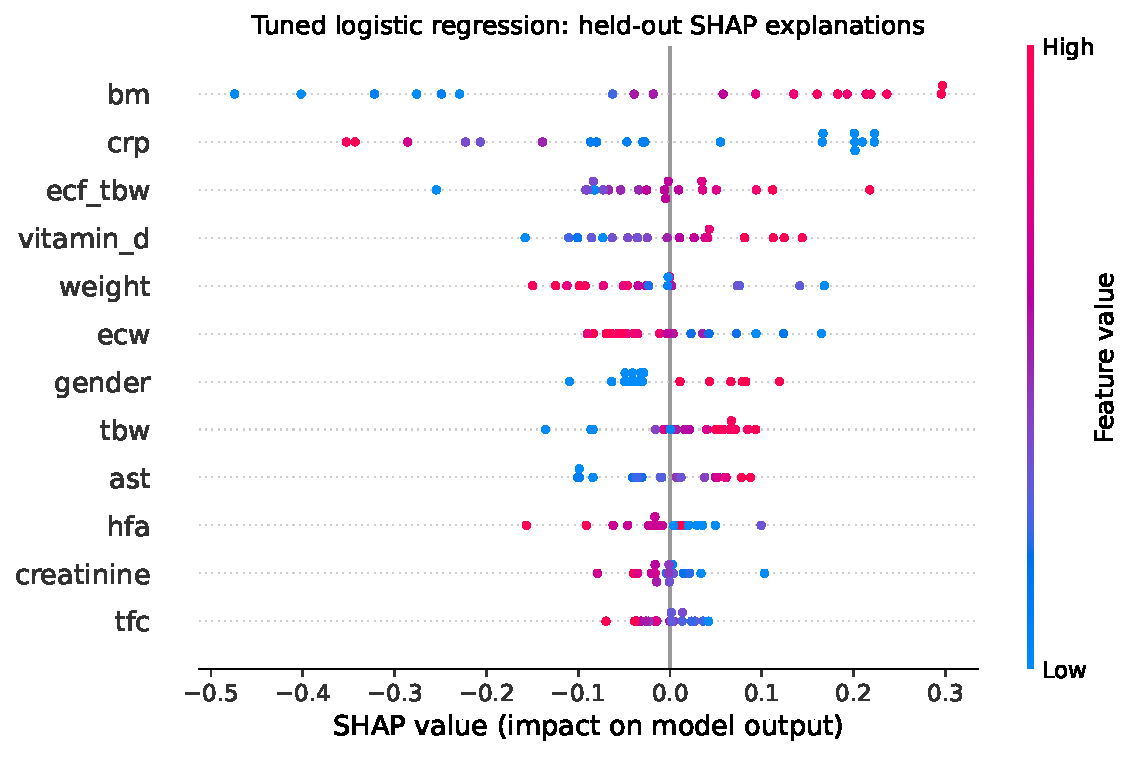
\includegraphics[width=0.88\linewidth]{figures/xai/global_shap.pdf}
\caption{Kernel SHAP summary for 20 sampled excluded records from tuned logistic Leave One Patient Out models. Each point uses its own outer-fold model and training-only background. Positive values increase the predicted probability of gallstones; negative values decrease it. Colour indicates the recorded feature value, and source-field labels follow the dataset schema. Features are ordered by sampled mean absolute contribution.}
\label{fig:xai-global}
\end{figure}

Figure~\ref{fig:xai-errors} compares SHAP and LIME for two confident errors. Source record 156 was a false negative with predicted probability 0.038; its largest displayed negative SHAP contributions included fluid ratio, \texttt{bm}, and vitamin D. Source record 178 was a false positive with predicted probability 0.995. These examples illustrate how multiple contributions can support an incorrect prediction despite aggregate discrimination. SHAP baselines were 0.443 and 0.413, respectively, and reconstruction from all feature contributions matched the saved probabilities. Only the eight largest contributions are displayed locally.

LIME surrogate $R^2$ was 0.423 for the false negative and 0.230 for the false positive, indicating limited local fidelity. For record 156, the surrogate prediction (0.160) also differed from the classifier probability (0.038). LIME condition weights and SHAP probability contributions have different meanings and should not be compared numerically. Agreement in direction is descriptive; correlated measurements and synthetic perturbations can produce unstable or implausible neighbourhoods.

\begin{figure*}[t]
\centering
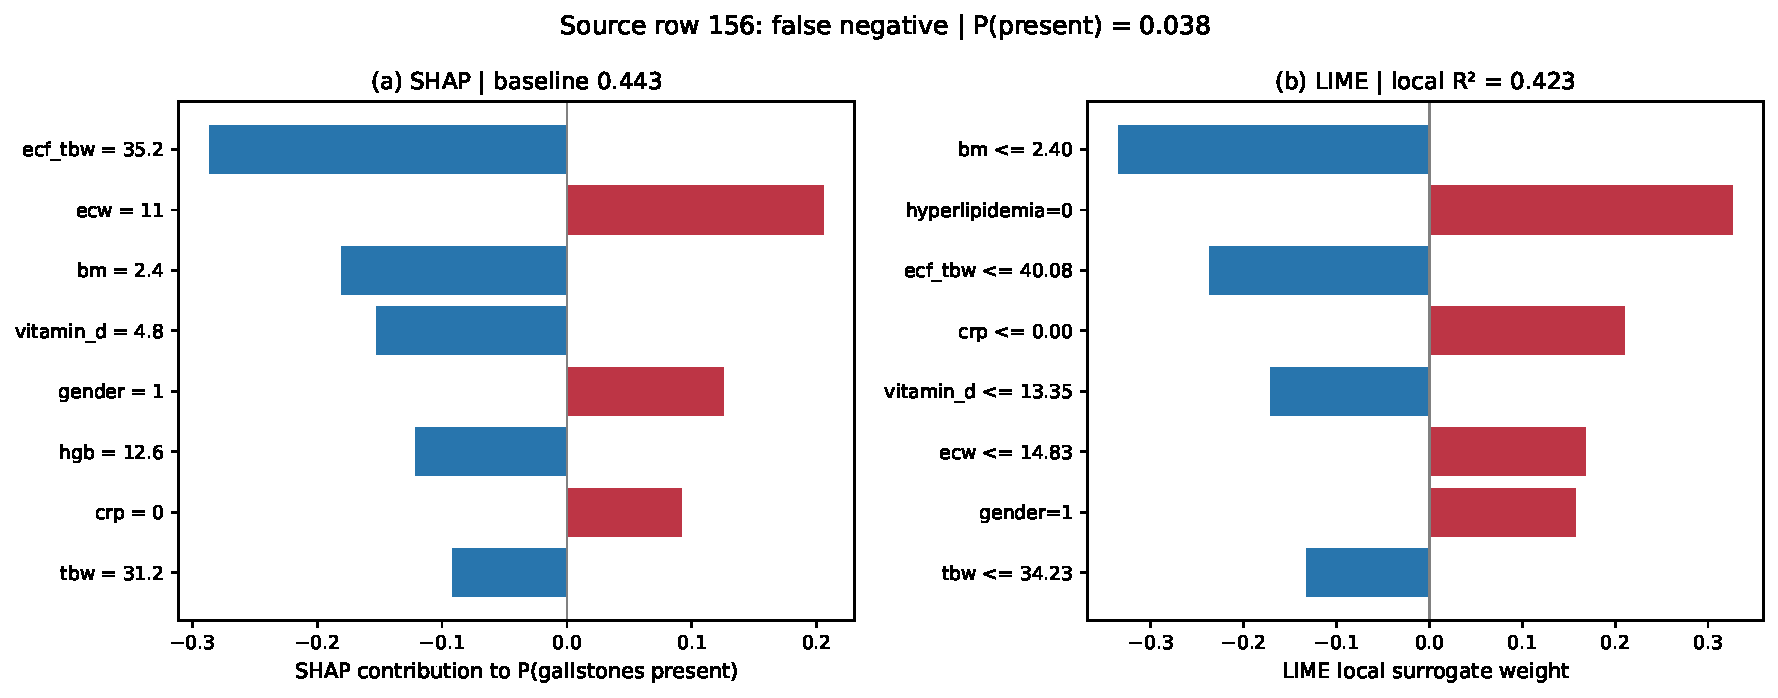
\includegraphics[width=0.88\linewidth]{figures/xai/local_fn.pdf}
\par\medskip
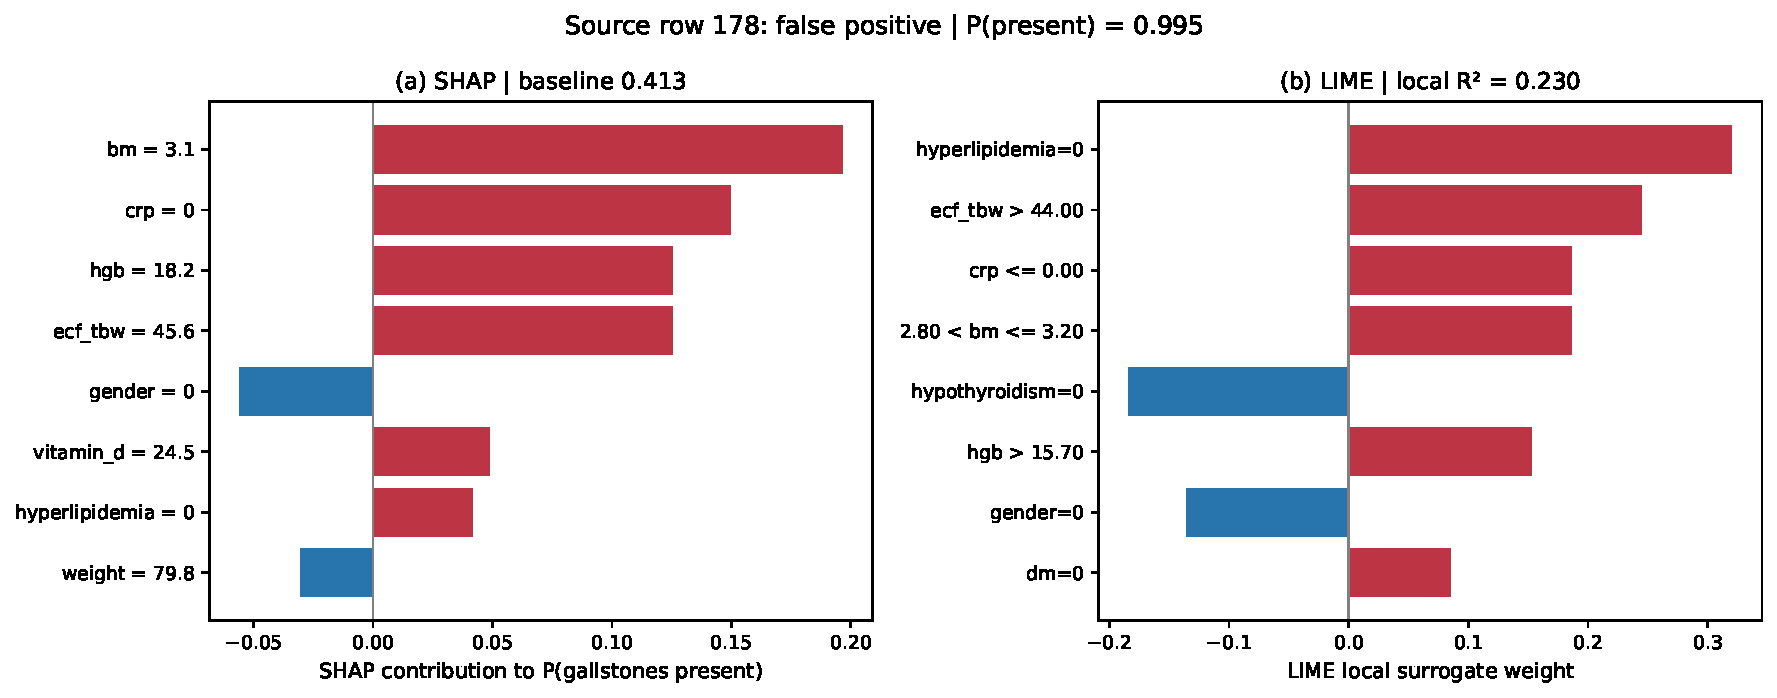
\includegraphics[width=0.88\linewidth]{figures/xai/local_fp.pdf}
\caption{Local explanations of a retrospectively selected false negative (source row 156, top) and false positive (source row 178, bottom) from tuned logistic Leave One Patient Out evaluation. Left: the eight largest absolute SHAP contributions, labelled with recorded input values. Right: LIME condition weights and local surrogate fidelity. Red pushes towards gallstones present; blue pushes towards absent. Each excluded record was omitted from fitting, tuning, and explainer background construction. These selected examples do not estimate error prevalence.}
\label{fig:xai-errors}
\end{figure*}


\section{Discussion}\label{sec:discussion}
\subsection{Principal findings}
Logistic regression achieved the strongest pooled discrimination in the historical fixed and fixed-feature tuned comparisons. Within the tuned families, it also achieved the highest F1 and matched XGBoost's sensitivity. The historical fixed random forest had higher sensitivity than its tuned counterpart, while tuning improved XGBoost's descriptive AUC and classification outcomes. LightGBM and stacking offered the highest tuned specificity. These trade-offs show that an inner-AUC search objective does not necessarily improve every outer metric, and that added complexity confers no uniform advantage. Dependency changes prevent attributing historical before/after differences solely to tuning; the observed rankings do not establish statistically significant superiority.

The updated base-tuned stack subsequently achieved AUC 0.8762 and F1 0.8133, with 26 false negatives, improving descriptively over its historical tuned counterpart. Jointly changing the base learners, their tuning, feature-count search and sampler scheduling prevents isolating the cause. The standalone candidates have not completed the same expanded feature-count search; shared outer exclusions and a common inner-CV budget do not by themselves make those configurations fully controlled comparators. Frequent selection of all 38 predictors also argues against presuming that feature reduction necessarily helps this architecture.

The findings accord with literature showing that optimisation and ensemble complexity do not consistently improve performance on Gallstone-1. Published scores cannot be compared directly with these LOPO estimates because training sizes, feature-selection procedures, thresholds, and assessment samples differ. Likewise, errors recurring across model families suggest shared limitations in the available measurements or fitted relationships, but retrospective inspection cannot determine a record's clinical circumstances or establish incorrect labels.

The additional SHAP and LIME analysis offers a visual account of model reliance and confident errors. Its global summary uses only 20 excluded records, and local examples were selected after observing errors. Modest LIME fidelity limits the strength of patient-specific interpretation. Neither method validates biological mechanisms or resolves errors; larger explanatory samples and stability analyses would be needed to assess robustness.

\subsection{Limitations}
The analysis relies on a small cohort from one clinical setting. Its near-balanced case distribution does not establish predictive values or assessment workload in populations with different prevalence. Availability of detailed bioimpedance measurements may further constrain transferability. Source-row identifiers are not verified person identifiers; the LOPO interpretation assumes one record per person, and repeated-person data would require grouped exclusion.

Fold-specific preprocessing prevents direct use of excluded records during fitting, but the analysis evaluates fixed pipelines and within-family nested tuning rather than the entire model-development process. The dataset and modelling choices had been explored previously; consequently, LOPO is an internal comparison rather than an untouched confirmatory assessment. Retrospective selection of the strongest family can introduce optimism, and the heavily overlapping training folds are not independent experiments. The single fixed-seed run does not quantify random-state variability or furnish confidence intervals for model differences.

The study did not establish calibrated probabilities, optimise a clinical operating threshold, or demonstrate external generalisation or clinical benefit. Feature selection may also vary across folds because correlated measurements can substitute for one another. Aggregate metrics and recurring error examples therefore require cautious interpretation and do not establish causal relationships.

\subsection{Implications for further research}
The implemented tuning nests parameter selection within outer training sets. Further work should extend this boundary to model-family choice, feature-count decisions, calibration, and operating-threshold selection. A sensitivity-oriented threshold should be assessed jointly with specificity and assessment workload. Grouped feature ablation and prespecified subgroup evaluation could investigate measurement burden and uneven errors. An untouched external cohort is required to assess transfer beyond this dataset. Prospective disease-onset prediction would require a different study design and outcome definition.


\section{Conclusion}\label{sec:conclusion}
Under a shared Leave One Patient Out framework, tuned logistic regression provided the strongest discrimination and F1, while matching XGBoost's sensitivity. LightGBM and stacking offered the highest tuned specificity. XGBoost showed the largest descriptive improvement over its historical fixed configuration; tuning did not consistently improve the remaining families. Fold-specific preparation and nested parameter selection provide a reproducible internal benchmark, while SHAP and LIME expose model reliance and confident errors. Historical environment differences, prior cohort exploration, retrospective family comparison, and absent external validation restrict these findings to comparative research on existing gallstone status.


\section*{Data and Code Availability}
The data originate from the UCI Gallstone dataset \parencite{uci2025gallstone}. The manuscript source, Python workflow, notebooks, and saved experimental outputs are available at \url{https://github.com/QuyDuong106/INFOSYS722_Experimental}. Completed nested Optuna evidence is stored separately for each model family under \texttt{results/optuna\_MODEL/}; configurations, outer-fold predictions, and trial histories support reproduction of the reported metrics.

% \section*{Use of Artificial Intelligence}
% Generative artificial intelligence tools were used to assist language editing, LaTeX formatting, and manuscript organisation and restructuring.

\bibliographystyle{IEEEtranN}
\bibliography{references}
\end{document}
